\documentclass{assets/seminarpaper}

% +-----------------------------------------+ %
% | ADD PACKAGES HERE IF YOU NEED THEM      | %
% +-----------------------------------------+ %
\usepackage[T1]{fontenc}
\usepackage[protrusion=true,expansion=false]{microtype}
\usepackage{booktabs}
\usepackage{mathtools}
\usepackage{amssymb}
\usepackage{array}
\usepackage{float}
\DeclareMathOperator*{\argmin}{arg\,min}

% +-----------------------------------------+ %
% | FILL OUT PARAMETERS                     | %
% +-----------------------------------------+ %
\seminar{Seminar CurrAI}
\title{Symmetry as a Design Axis in Variational Quantum Learning}
\author{Markus Baumann}
\supervisor{Jonas Stein}
\abstract{%
Diese Arbeit untersucht Symmetrie als induktiven Bias in Variational Quantum Learning. Ausgangspunkt ist Meyer et al., die zeigen, dass ein $D_4$-äquivariantes Tic-Tac-Toe-Modell besser generalisieren kann als ein unbeschränktes Modell. Die Arbeit rekonstruiert diese Idee, erweitert sie aber um zwei experimentelle Fragen: Erstens wird die volle Symmetrie nicht nur gegen keine Symmetrie, sondern gegen Untergruppen wie $C_4$, $D_2$ und $Z_2$ verglichen. Zweitens wird untersucht, ob die größte Verbesserung nicht durch mehr oder weniger Symmetrie, sondern durch eine besser zur Aufgabe passende äquivariante Gate-Struktur entsteht. Dazu werden die ursprünglichen gerichteten Edge-Interaktionen um trainierbare Winning-Line-Gates auf den acht Gewinnlinien des Spielfelds erweitert. Die finalen 10-Seed-Experimente reproduzieren den Meyer-artigen Generalisierungseffekt: $D_4$ verbessert die Test Accuracy gegenüber keiner Symmetrie und reduziert den Generalization Gap. Partielle Symmetrie, insbesondere $C_4$, erreicht fast dieselbe Leistung wie $D_4$, schlägt es aber nicht robust. Der stärkste empirische Effekt kommt von task-aligned equivariant gates: ein $D_4$-äquivariantes Edge-plus-Line-Modell erreicht bei 600 Trainingsbeispielen etwa $0.785$ Test Accuracy gegenüber etwa $0.687$ für den Meyer-artigen Edge-Ansatz. Parameter-matched random sharing zeigt, dass der Effekt nicht bloß durch weniger Parameter erklärt wird. Die Schlussfolgerung ist konservativ: Die Arbeit behauptet keinen Quantum Advantage, sondern zeigt an einem kontrollierten Benchmark, dass Äquivarianz nicht nur als harte Constraint, sondern als Architekturprinzip verstanden werden sollte.
}

\begin{document}

\maketitle

% +-----------------------------------------+ %
% | ADD YOUR TEXT IN contents.tex           | %
% +-----------------------------------------+ %
\section{Einleitung}\label{sec:einleitung}

Symmetrie ist einer der wenigen induktiven Biases, die gleichzeitig mathematisch präzise, architektonisch umsetzbar und empirisch überprüfbar sind. Wenn eine Lernaufgabe invariant gegenüber einer Transformation ist, sollte ein Modell diese Invarianz nicht erst aus endlich vielen Daten lernen müssen. Bei Bildern führt diese Idee zu Faltungen und gruppenäquivarianten Netzen~\cite{lecun1998gradient,cohen2016group}; bei Mengen führt sie zu permutationsinvarianten Architekturen wie Deep Sets~\cite{zaheer2017deep}; im allgemeineren geometrischen Deep Learning wird sie als Grundprinzip formuliert, Datenräume, Gruppenwirkungen und Modellklassen gemeinsam zu betrachten~\cite{bronstein2021geometric}.

Für Variational Quantum Machine Learning ist diese Perspektive besonders relevant. Variational Quantum Learning Models (VQLMs) bestehen aus parametrisierten Quantenschaltkreisen, deren Erwartungswerte als Vorhersagen interpretiert werden~\cite{benedetti2019parameterized,schuld2020circuit}. Sie sind flexibel, aber diese Flexibilität ist ambivalent. Auf NISQ-Geräten sind Schaltkreistiefe, Messstatistik und Rauschen begrenzt~\cite{preskill2018quantum,bharti2022noisy}. Zudem kann hohe Expressivität die Optimierung erschweren und Generalisierung verschlechtern~\cite{mcclean2018barren,pesah2021absence}. Ein sinnvoller architektonischer Bias ist deshalb nicht nur ästhetisch, sondern praktisch notwendig.

Der Ausgangspunkt dieser Arbeit ist das Paper \emph{Exploiting symmetry in variational quantum machine learning} von Meyer et al.~\cite{meyer2022exploiting}. Die Autoren zeigen, wie eine bekannte Datensymmetrie in ein VQLM eingebaut werden kann. Im Tic-Tac-Toe-Beispiel ist das Label invariant unter den acht Rotationen und Spiegelungen des Spielfelds, also unter der Diedergruppe $D_4$. Meyer et al. konstruieren ein Modell, dessen Vorhersage diese Symmetrie per Konstruktion respektiert, und zeigen qualitativ, dass das symmetrische Modell besser generalisieren kann als ein unbeschränktes Modell.

Diese Arbeit übernimmt diese Idee, verschiebt aber die Fragestellung. Meyer et al. beantworten die Frage, ob volle Symmetrie gegenüber keiner Symmetrie helfen kann. Die natürliche Anschlussfrage lautet: Ist die volle Symmetrie bereits das Ende des Designraums? Oder kann man innerhalb der Klasse symmetrieverträglicher Modelle noch bessere Architekturen bauen? Genau hier liegt der Beitrag dieser Arbeit. Symmetrie wird nicht nur als Ja-Nein-Entscheidung verstanden, sondern als Architekturprinzip mit mehreren Freiheitsgraden.

Wir untersuchen drei Ebenen. Erstens reproduzieren wir den Meyer-artigen Effekt auf dem Tic-Tac-Toe-Benchmark: Ein $D_4$-äquivariantes Modell generalisiert besser als ein Modell ohne Parameter-Sharing. Zweitens ersetzen wir die binäre Gegenüberstellung von \emph{none} und $D_4$ durch eine Familie von Untergruppenmodellen: $Z_2$-Rotation, $Z_2$-Spiegelung, $C_4$, $D_2$ und volles $D_4$. Dadurch wird partielle Äquivarianz als diskreter Regler zwischen Expressivität und induktivem Bias sichtbar. Drittens führen wir task-aligned equivariant gates ein: trainierbare Gates auf den acht Gewinnlinien des Tic-Tac-Toe-Felds. Diese Gates brechen die Symmetrie nicht, sondern respektieren sie über dasselbe Orbit-Sharing. Sie geben dem Schaltkreis aber direkten Zugriff auf die dreizelligen Motive, aus denen das Label berechnet wird.

Die wichtigsten Ergebnisse sind konservativ, aber klar. Die Reproduktion bestätigt die Richtung von Meyer et al.: Bei Trainingsgröße 450 erreicht das unbeschränkte Edge-Modell $0.614\pm0.029$ Test Accuracy, während das $D_4$-äquivariante Edge-Modell $0.688\pm0.036$ erreicht. Der Generalization Gap sinkt von $0.094$ auf $0.023$. Die partielle Symmetrie $C_4$ erreicht fast dieselbe Leistung wie $D_4$ und liegt in einzelnen Low-Data-Regimen leicht vorn, aber nicht robust genug für den Claim, dass weniger Symmetrie grundsätzlich besser sei. Der stärkste Effekt entsteht durch die winning-line gates: Das beste $D_4$-äquivariante Edge-plus-Line-Modell erreicht etwa $0.80$ Test Accuracy, also deutlich mehr als der Meyer-artige Edge-Ansatz mit etwa $0.69$.

Die Arbeit behauptet keinen Quantum Advantage. Tic-Tac-Toe ist klassisch trivial; ein deterministischer Regel-Oracle erreicht auf allen 5478 legalen Zuständen 100\% Genauigkeit mit null trainierbaren Parametern. Gerade deshalb ist der Benchmark nützlich: Er erlaubt eine kontrollierte Untersuchung, ob ein VQLM die bekannte Struktur sinnvoll nutzt. Die wissenschaftliche Aussage ist nicht, dass ein Quantenmodell Tic-Tac-Toe besonders gut löst. Die Aussage ist, dass Äquivarianz in VQLMs nicht nur eine Parameterreduktion ist, sondern ein Designprinzip dafür, welche trainierbaren Interaktionen überhaupt angeboten werden sollten.

\section{Theoretischer Hintergrund}\label{sec:theorie}

\subsection{Variational Quantum Learning Models}\label{subsec:vqlm}

Ein VQLM kodiert klassische Daten $x$ in einen Quantenzustand, verarbeitet diesen Zustand mit trainierbaren Gates und liest Erwartungswerte von Observablen aus. Eine typische Vorhersage hat die Form
\begin{equation}
f_\theta(x)=
\langle 0|U^\dagger_\theta(x) O U_\theta(x)|0\rangle,
\label{eq:vqlm}
\end{equation}
wobei $O$ ein Observable und $U_\theta(x)$ ein datenabhängiger parametrisierter Schaltkreis ist. In Data-Reuploading-Modellen wird dasselbe Daten-Encoding mehrfach in den Schaltkreis eingebracht~\cite{perez2020data}. Dadurch kann das Modell nichtlineare Funktionen der Eingabe darstellen. Eine typische Form ist
\begin{equation}
U_\theta(x)=W_L(\theta)U(x)\cdots W_1(\theta)U(x),
\label{eq:reuploading}
\end{equation}
wobei $U(x)$ das Daten-Encoding und $W_\ell(\theta)$ trainierbare Blöcke sind.

Die zentrale Designfrage ist nicht nur, wie viele Parameter ein solcher Schaltkreis hat. Entscheidend ist, welche Funktionen durch Encoding, Gates und Messung erreichbar sind. Symmetrie wirkt genau auf diese Funktionsklasse. Wenn ein Modell invariant unter einer Gruppe $G$ sein soll, gilt
\begin{equation}
f_\theta(gx)=f_\theta(x)
\quad\text{für alle }g\in G.
\label{eq:invariance}
\end{equation}
Ein Modell, das diese Gleichheit per Konstruktion erfüllt, muss sie nicht aus Daten lernen. Das ist besonders in Low-Data-Regimen relevant.

\subsection{Von Datensymmetrien zu Hilbert-Raum-Repräsentationen}\label{subsec:repr}

Meyer et al. formulieren die Symmetriebedingung über eine kompatible Darstellung im Hilbert-Raum~\cite{meyer2022exploiting}. Eine Datentransformation $g$ soll durch einen unitären Operator $U_g$ so dargestellt werden, dass
\begin{equation}
U(gx)=U_g U(x) U_g^\dagger.
\label{eq:encoding-equivariance}
\end{equation}
Wenn zusätzlich der Startzustand und das Observable invariant sind und die trainierbaren Blöcke mit allen $U_g$ kompatibel sind, folgt die Invarianz der Vorhersage.

Im Tic-Tac-Toe-Beispiel ist diese Bedingung anschaulich. Jedes der neun Spielfeldfelder wird einem Qubit zugeordnet. Eine Rotation oder Spiegelung des Spielfelds ist dann eine Permutation der Qubits. Die Diedergruppe $D_4$ enthält acht Transformationen: Identität, Rotationen um $90^\circ$, $180^\circ$ und $270^\circ$, sowie vier Spiegelungen. Ecken werden auf Ecken abgebildet, Kanten auf Kanten, und das Zentrum bleibt Zentrum. Dadurch entstehen natürliche Orbits im Schaltkreis.

\subsection{Gate Symmetrization und Parameter-Sharing}\label{subsec:sharing}

Meyer et al. beschreiben Gate Symmetrization über Twirling. Ein Gate
\begin{equation}
R_G(\theta)=\exp(-i\theta G)
\end{equation}
ist symmetrieverträglich, wenn sein Generator $G$ mit der Gruppenrepräsentation kommutiert. Aus einem beliebigen Generator kann durch
\begin{equation}
\Pi_{\mathrm{sym}}(G)
=\frac{1}{|G|}\sum_{g\in G}U_g G U_g^\dagger
\label{eq:twirling}
\end{equation}
ein symmetrischer Anteil gewonnen werden. In unserer Implementierung verwenden wir für den Tic-Tac-Toe-Ansatz eine äquivalente und transparente Sicht: Parameter werden entlang der Orbits der Gruppe geteilt. Alle Qubits oder gerichteten Gate-Paare, die durch eine Symmetrie ineinander überführt werden, erhalten denselben trainierbaren Parameter.

Für volles $D_4$ bedeutet das zum Beispiel: alle vier Ecken teilen Parameter, alle vier Kanten teilen Parameter, und das Zentrum bleibt ein eigener Orbit. Für eine kleinere Untergruppe wie $C_4$ werden nur Rotationen erzwungen; Spiegelungen müssen nicht identisch behandelt werden. Damit entsteht ein diskreter Bias-Expressivitäts-Regler. Größere Untergruppen erzwingen mehr Gleichheiten und reduzieren die Zahl trainierbarer Parameter. Kleinere Untergruppen erlauben mehr Ausdruckskraft, verlieren aber einen Teil des induktiven Bias.

\section{Vom Originalpaper zur eigenen Fragestellung}\label{sec:fragestellung}

\subsection{Was Meyer et al. zeigen}\label{subsec:meyer}

Das Originalpaper zeigt, dass Symmetrie in VQLMs nicht nur nachträglich als Regularisierung formuliert werden muss, sondern direkt in den Schaltkreis eingebaut werden kann~\cite{meyer2022exploiting}. Am Tic-Tac-Toe-Benchmark ist die zentrale qualitative Beobachtung: Ein symmetrisches Modell kann eine niedrigere oder ähnliche Trainingsleistung haben, aber besser testen. Das freie Modell hat mehr Freiheitsgrade und kann Trainingsdaten stärker ausnutzen; das symmetrische Modell beschränkt sich auf Funktionen, die zur Aufgabenstruktur passen.

Diese Aussage ist wissenschaftlich sauber, aber sie lässt eine Anschlussfrage offen. Das Originalpaper behandelt Symmetrie im Tic-Tac-Toe-Beispiel im Wesentlichen als volle Task-Symmetrie. Sobald $D_4$ bekannt ist, liegt es nahe, die ganze Gruppe zu erzwingen. Aus Sicht der Modellarchitektur ist das aber nicht die einzige mögliche Entscheidung. Man kann Untergruppen erzwingen, Parameter randomisiert teilen, zusätzliche äquivariante Gates einbauen oder die Symmetrie nur als Loss-Regularisierung verwenden. Die interessante Frage ist daher nicht nur: \emph{Hilft Symmetrie?} Sondern: \emph{Welche symmetrieverträgliche Architektur hilft?}

\subsection{Research Question}\label{subsec:rq}

Die Arbeit untersucht die Frage:
\begin{quote}\small
Ist volle $D_4$-Äquivarianz die beste praktische Induktionsannahme im Tic-Tac-Toe-VQLM? Oder kann man durch partielle Symmetrie und task-aligned equivariant gates bessere Generalisierung erreichen?
\end{quote}

Daraus folgen drei Hypothesen:
\begin{enumerate}
\item Volles $D_4$ sollte gegenüber keiner Symmetrie besser generalisieren, weil es die korrekte Aufgabeninvarianz erzwingt.
\item Partielle Symmetrien, insbesondere $C_4$, könnten in einigen Regimen ähnlich gut oder leicht besser sein, weil sie mehr Expressivität erhalten.
\item Der größte Gewinn könnte nicht aus weniger oder mehr Symmetrie kommen, sondern aus einer besseren äquivarianten Gatelokalisierung: Winning-Line-Gates sollten dem Modell die entscheidenden Tic-Tac-Toe-Motive direkter zugänglich machen.
\end{enumerate}

Die dritte Hypothese ist die stärkste Erweiterung. Sie verschiebt den Fokus von \emph{symmetry as parameter reduction} zu \emph{symmetry as architecture design}. Die Frage ist dann nicht mehr nur, wie viele Parameter übrig bleiben, sondern ob die trainierbaren Interaktionen zur Kombinatorik der Aufgabe passen.

\subsection{Designraum}\label{subsec:designraum}

\Cref{fig:protocol} fasst den Designraum zusammen. Panel (a) zeigt die $D_4$-Symmetrie des Spielfelds. Panel (b) zeigt die Datenkodierung und die durch Untergruppen induzierten Orbits. Panel (c) zeigt den Unterschied zwischen dem Meyer-artigen Edge-Ansatz und unserer winning-line-Erweiterung. Wichtig ist: Die Erweiterung ist kein symmetry breaking. Die zusätzlichen Gates werden ebenfalls über Gruppenorbits geteilt und bleiben daher äquivariant.

\begin{figure}[t]
\centering
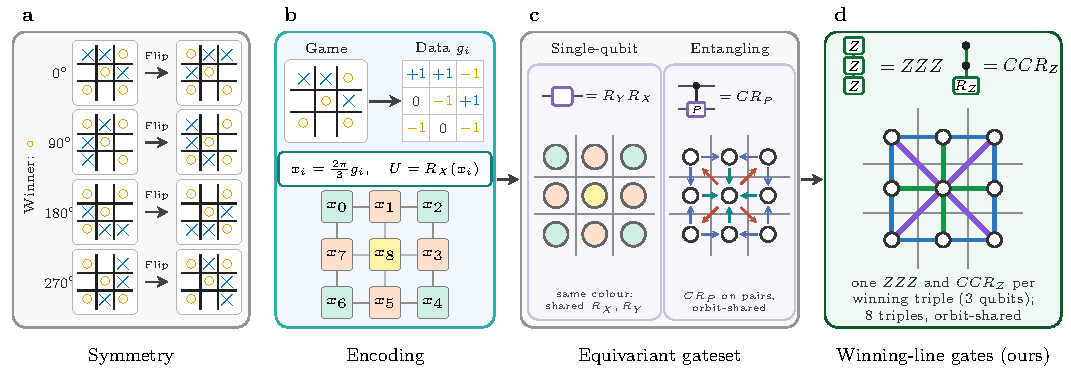
\includegraphics[width=\textwidth]{images/fig_protocol.pdf}
\caption{Designraum der Arbeit. Ausgehend von der $D_4$-Symmetrie des Tic-Tac-Toe-Bretts werden Daten auf neun Qubits kodiert. Untergruppen erzeugen unterschiedliche Parameter-Sharing-Orbits. Die eigene Erweiterung ergänzt den Meyer-artigen Edge-Ansatz um Gates auf den acht Gewinnlinien, ohne die Äquivarianz zu brechen.}
\label{fig:protocol}
\end{figure}

\section{Experimentelles Protokoll}\label{sec:protokoll}

\subsection{Datensatz und Labels}\label{subsec:dataset}

Wir erzeugen alle legal erreichbaren Tic-Tac-Toe-Zustände aus dem Spielbaum. Ein Spielfeld wird mit neun Positionen dargestellt:
\[
\begin{matrix}
0 & 1 & 2\\
7 & 8 & 3\\
6 & 5 & 4
\end{matrix}.
\]
Die Ecken sind $\{0,2,4,6\}$, die Kanten $\{1,3,5,7\}$, und das Zentrum ist $8$. Jedes Feld hat den Wert $+1$ für Kreuz, $-1$ für Kreis und $0$ für leer. Die Klassen sind Circle Win, Draw und Cross Win. Wie im Originalsetting werden auch unfertige Spiele als Draw gelabelt, weil kein Gewinner feststeht. Die Labelvektoren sind
\[
y_{\mathrm{circle}}=(+1,-1,-1),\quad
y_{\mathrm{draw}}=(-1,+1,-1),\quad
y_{\mathrm{cross}}=(-1,-1,+1).
\]
Trainings- und Testsets werden pro Seed balanciert und disjunkt gesampelt. Die Standardgröße für die Reproduktion ist 450 Trainingsbeispiele und 600 Testbeispiele.

\subsection{Schaltkreis}\label{subsec:circuit}

Das Modell verwendet neun Qubits. Für jeden Datenpunkt wird auf Qubit $i$ die Rotation
\begin{equation}
R_X(2\pi x_i/3)
\label{eq:encoding}
\end{equation}
angewendet. Diese Datenkodierung wird in jedem Layer re-uploaded. Der trainierbare Standardblock besteht aus Single-Qubit-Rotationen und gerichteten CRY-Gates. Die gerichteten Paare folgen der Brettgeometrie: Kanten zwischen benachbarten Ecken und Kantenfeldern, Kante-Zentrum-Verbindungen und Zentrum-Ecke-Verbindungen.

Die Vorhersage ist ein dreidimensionaler Erwartungswertvektor:
\begin{equation}
\hat y(x)=
\left(
\frac{1}{4}\sum_{i\in C}\langle Z_i\rangle,\;
\langle Z_8\rangle,\;
\frac{1}{4}\sum_{i\in E}\langle Z_i\rangle
\right),
\label{eq:readout}
\end{equation}
wobei $C=\{0,2,4,6\}$ und $E=\{1,3,5,7\}$. Die vorhergesagte Klasse ist die Komponente mit dem größten Erwartungswert. Optimiert wird der Mean Squared Error zwischen $\hat y(x)$ und dem Labelvektor.

Sofern nicht anders angegeben, verwenden die Experimente $L=3$ Reuploading-Layer, $p=2$ Wiederholungen des trainierbaren Blocks pro Layer, Batchgröße 15, 30 Minibatch-Schritte pro Epoche, 100 Epochen und Adam mit Lernrate $0.01$. Alle dargestellten Hauptergebnisse sind Mittelwerte über fünf Seeds mit 95\%-Konfidenzintervallen.

\subsection{Untergruppen und Parameterzahlen}\label{subsec:groups}

Die sechs untersuchten Sharing-Varianten sind in \Cref{tab:groups} dargestellt. Die Topologie des Edge-Schaltkreises bleibt dabei gleich; nur das Parameter-Sharing ändert sich. Dadurch ist der Vergleich sauberer als ein Vergleich vollständig verschiedener Schaltkreise.

\begin{table}[t]
\centering
\caption{Untersuchte Symmetrievarianten im Meyer-artigen Edge-Ansatz bei $L=3,p=2$.}
\label{tab:groups}
\begin{tabular}{lccc}
\toprule
Variante & Kategorie & Ordnung & Parameter\\
\midrule
none & keine Symmetrie & 1 & 204\\
$Z_2$ rotation & partiell & 2 & 108\\
$Z_2$ reflection & partiell & 2 & 126\\
$C_4$ & partiell & 4 & 60\\
$D_2$ & partiell & 4 & 78\\
$D_4$ & voll & 8 & 54\\
\bottomrule
\end{tabular}
\end{table}

Diese Tabelle zeigt bereits einen wichtigen Punkt. Mehr Symmetrie bedeutet in diesem Ansatz weniger Parameter. Das heißt aber nicht, dass jede Verbesserung automatisch durch weniger Parameter erklärt ist. Dafür benötigen wir einen Random-Sharing-Control: Für jede symmetriegebundene Parameterzahl wird ein zufälliges, type-preserving Sharing erzeugt, das ungefähr gleich viele Parameter besitzt, aber keine Gruppenstruktur respektiert.

\subsection{Winning-Line-Gates}\label{subsec:linegates}

Der Meyer-artige Edge-Ansatz verwendet lokale gerichtete Paare. Tic-Tac-Toe-Gewinne entstehen jedoch nicht aus beliebigen lokalen Paaren, sondern aus acht Dreierlinien: drei Zeilen, drei Spalten und zwei Diagonalen. Deshalb testen wir zusätzliche trainierbare Interaktionen auf diesen Triples. Die wichtigsten Familien sind:
\begin{itemize}
\item \texttt{line\_zzz}: MultiRZ-artige $ZZZ$-Rotationen auf Gewinnlinien,
\item \texttt{line\_ccrz}: symmetrische controlled-controlled-$R_Z$-Interaktionen,
\item \texttt{line\_zzz\_ccrz}: Kombination beider Line-Gates,
\item \texttt{edge\_line\_zzz\_ccrz}: Edge-Ansatz plus beide Winning-Line-Kanäle.
\end{itemize}
Auch diese Parameter werden über $C_4$- oder $D_4$-Orbits geteilt. Die beste Familie ist also weiterhin äquivariant; sie ist nur stärker an die Aufgabenlogik angepasst.

\section{Ergebnisse}\label{sec:ergebnisse}

\subsection{Reproduktion: volle Symmetrie generalisiert besser}\label{subsec:repro}

\Cref{fig:main} zeigt die zentrale Evidenz. Die Reproduktion bestätigt die erwartete Richtung. Das unbeschränkte Edge-Modell erreicht bei 450 Trainingsbeispielen $0.614\pm0.029$ Test Accuracy. Das $D_4$-äquivariante Edge-Modell erreicht $0.688\pm0.036$. Gleichzeitig sinkt der Generalization Gap von $0.094$ auf $0.023$. Das freie Modell besitzt mit 204 Parametern deutlich mehr Freiheitsgrade als das $D_4$-Modell mit 54 Parametern, aber diese zusätzlichen Freiheitsgrade helfen auf dem Testset nicht.

\begin{figure}[t]
\centering
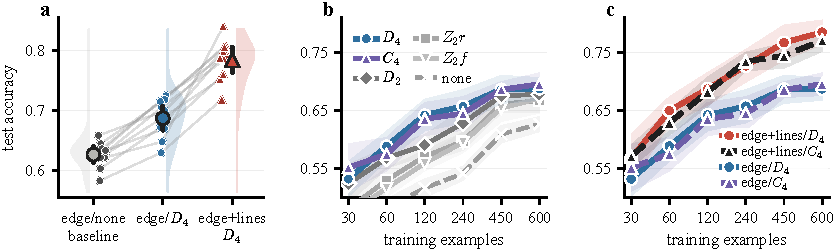
\includegraphics[width=\textwidth]{images/fig_main_evidence.pdf}
\caption{Hauptergebnisse. Links: Reproduktion des Meyer-artigen Effekts, $D_4$ schlägt keine Symmetrie. Mitte: Untergruppen-Sweep über Trainingsgrößen; $C_4$ folgt $D_4$ sehr eng. Rechts: Winning-Line-Gates verbessern die Accuracy deutlich, während der deterministische Regel-Oracle als 100\%-Referenz dient.}
\label{fig:main}
\end{figure}

Das ist genau das Muster eines sinnvollen induktiven Bias. Die Symmetrie reduziert die Hypothesenklasse nicht beliebig, sondern in einer Weise, die zur Aufgabenstruktur passt. Das Modell muss nicht lernen, dass eine gedrehte Gewinnstellung dasselbe Label hat; diese Gleichheit ist eingebaut.

\subsection{Partielle Äquivarianz: \texorpdfstring{$C_4$}{C4} ist konkurrenzfähig, aber kein robuster Sieger}\label{subsec:partial}

Der Untergruppen-Sweep zeigt ein differenzierteres Bild als ein reines none-vs-$D_4$-Experiment. In \Cref{tab:partial} sind die wichtigsten Werte zusammengefasst. $C_4$ erreicht über alle Datenregime hinweg fast dieselbe mittlere Test Accuracy wie $D_4$: $0.6149$ gegenüber $0.6152$. Bei 30 Trainingsbeispielen liegt $C_4$ mit $0.552$ über $D_4$ mit $0.531$; bei 120 Beispielen liegen beide praktisch gleichauf; bei 450 Beispielen erreichen $C_4$ und $D_4$ $0.689$ und $0.688$.

\begin{table}[t]
\centering
\caption{Partielle Äquivarianz im Edge-Ansatz. Werte sind mittlere Test Accuracy über fünf Seeds.}
\label{tab:partial}
\begin{tabular}{lcccc}
\toprule
Gruppe & Parameter & Test@30 & Test@450 & Mean Test\\
\midrule
none & 204 & 0.443 & 0.614 & 0.524\\
$Z_2$ rot & 108 & 0.495 & 0.677 & 0.572\\
$Z_2$ refl & 126 & 0.481 & 0.678 & 0.566\\
$C_4$ & 60 & 0.552 & 0.689 & 0.615\\
$D_2$ & 78 & 0.550 & 0.666 & 0.597\\
$D_4$ & 54 & 0.531 & 0.688 & 0.615\\
\bottomrule
\end{tabular}
\end{table}

\Cref{fig:lowdata} zeigt den Low-Data-Zoom für $C_4-D_4$. Die Interpretation sollte vorsichtig sein. Es gibt kleine Bereiche, in denen $C_4$ etwas besser ist. Das reicht nicht für die Aussage, dass $C_4$ allgemein besser sei. Es reicht aber für eine interessante praktische Aussage: Rotation-only Equivariance kann auf diesem Benchmark fast denselben Nutzen liefern wie volle $D_4$-Equivariance, obwohl Spiegelungsconstraints gelockert werden. Der Nutzen der vollen Gruppe ist also nicht als binäres Dogma zu verstehen.

\begin{figure}[t]
\centering
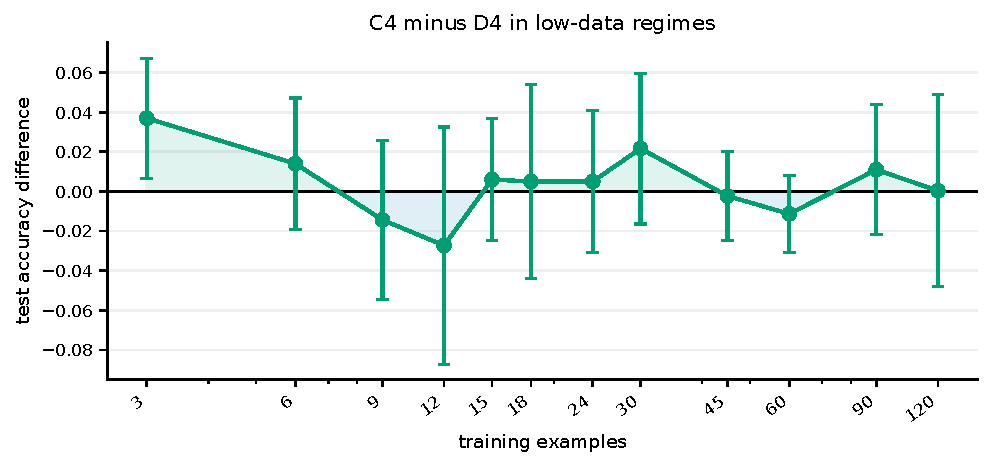
\includegraphics[width=0.82\textwidth]{images/fig_lowdata_delta.pdf}
\caption{Low-Data-Zoom: Differenz der Test Accuracy zwischen $C_4$ und $D_4$. Positive Werte bedeuten einen Vorteil für $C_4$. Die Vorteile sind klein und nicht robust genug für einen Dominanzclaim, zeigen aber, dass partielle Symmetrie eine sinnvolle Modellwahlachse ist.}
\label{fig:lowdata}
\end{figure}

\subsection{Random-Sharing-Control: Nicht nur weniger Parameter}\label{subsec:random}

Ein naheliegender Einwand lautet: Vielleicht hilft Symmetrie gar nicht als Struktur, sondern nur als Parameterreduktion. Dann wäre jedes zufällige Sharing mit derselben Parameterzahl ähnlich gut. Genau deshalb ist der Random-Sharing-Control wichtig. \Cref{fig:random} zeigt, dass dieser Einwand nicht ausreicht. Bei $D_4$ erreicht symmetry-aware sharing $0.688$, random sharing mit gleicher Parameterzahl aber nur $0.572$. Bei $C_4$ erreicht symmetry-aware sharing $0.689$, random sharing nur $0.551$.

\begin{figure}[t]
\centering
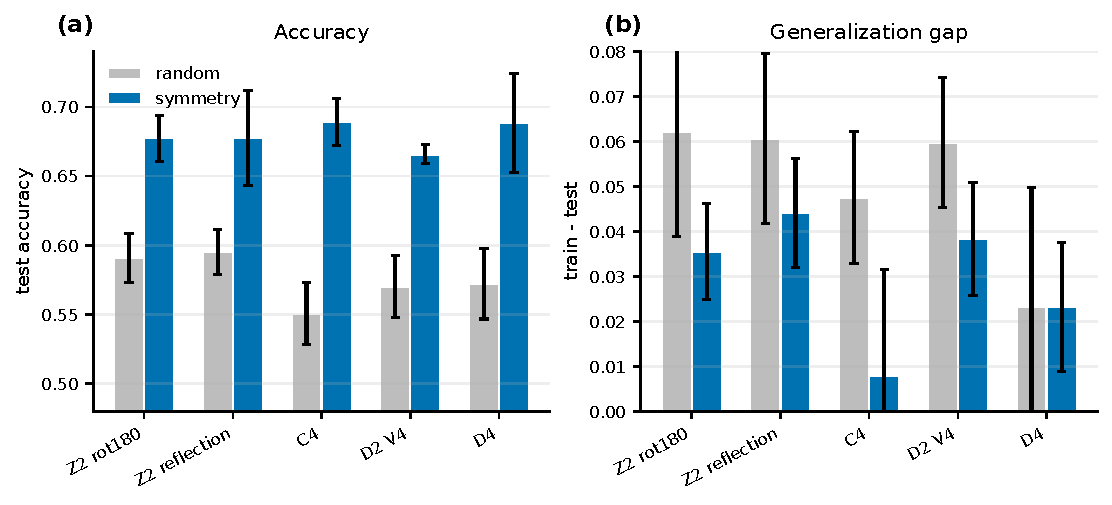
\includegraphics[width=0.82\textwidth]{images/fig_random_control.pdf}
\caption{Parameter-matched random sharing. Die zufällig geteilten Modelle haben ungefähr dieselbe Parameterzahl wie die jeweiligen Symmetriemodelle, respektieren aber keine Gruppenorbits. Die deutlich schlechtere Test Accuracy zeigt, dass der Effekt nicht bloß eine Folge kleinerer Modelle ist.}
\label{fig:random}
\end{figure}

Damit wird die zentrale Interpretation stärker. Die Verbesserung kommt nicht nur daher, dass Parameter entfernt werden. Sie kommt daher, dass Parameter entlang sinnvoller geometrischer Orbits geteilt werden. Das ist die gleiche Logik wie bei Faltungen: Ein CNN ist nicht nur kleiner als ein fully connected Netzwerk; seine Gewichtsteilung entspricht einer Strukturannahme über Bilder.

\subsection{Task-Aligned Equivariant Gates: der stärkste Effekt}\label{subsec:oracle}

Der deutlichste empirische Gewinn entsteht durch die winning-line gates. \Cref{fig:oracle} zeigt die robuste Auswertung für Trainingsgrößen 450, 600 und 750. Das Meyer-artige Edge/$D_4$-Modell liegt bei etwa $0.69$ bis $0.70$ Test Accuracy. Das beste Edge-plus-Line-Modell, \texttt{edge\_line\_zzz\_ccrz}/$D_4$, erreicht $0.795\pm0.016$ bei 450 Trainingsbeispielen und $0.805\pm0.019$ bei 600 Trainingsbeispielen. Bei 750 Beispielen fällt der Mittelwert auf $0.774$, bleibt aber deutlich über dem Edge-Baseline-Niveau.

\begin{figure}[t]
\centering
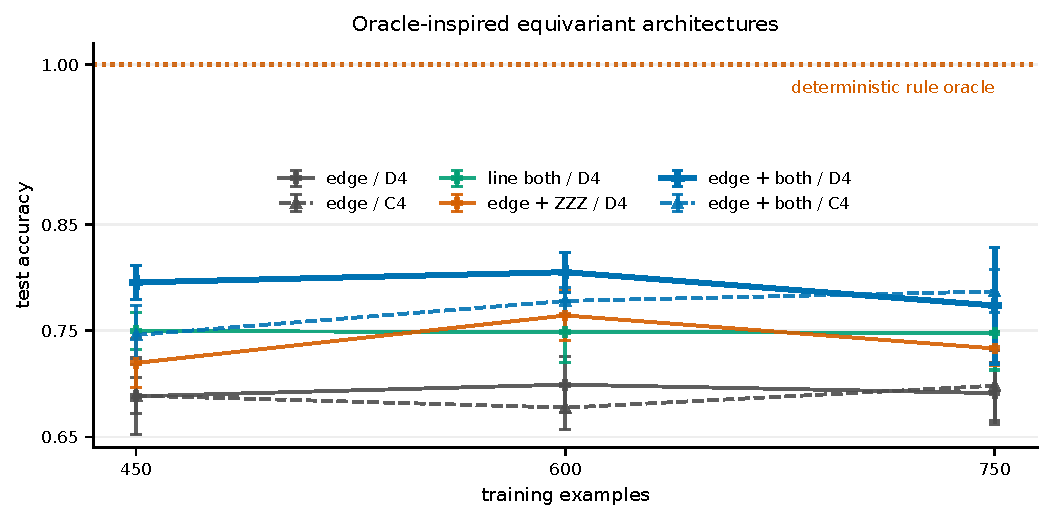
\includegraphics[width=\textwidth]{images/fig_oracle_accuracy.pdf}
\caption{Oracle-inspirierte äquivariante Architekturen. Die gestrichelte Linie bei 1.0 ist der deterministische Regel-Oracle und dient nur als obere Referenz. Die beste trainierbare Architektur kombiniert den Edge-Ansatz mit beiden Winning-Line-Kanälen und bleibt $D_4$-äquivariant.}
\label{fig:oracle}
\end{figure}

\Cref{fig:controls} zeigt die Ablationen. Line-Gates allein helfen teilweise, aber die beste Architektur kombiniert die ursprünglichen Edge-Interaktionen mit beiden Winning-Line-Kanälen. Das ist plausibel: Die Edge-Gates modellieren lokale Brettgeometrie und Zentrumskopplung, während die Line-Gates die tatsächlichen Gewinnmotive repräsentieren. Die Kombination gibt dem Modell sowohl lokale als auch regelnahe Struktur.

\begin{figure}[t]
\centering
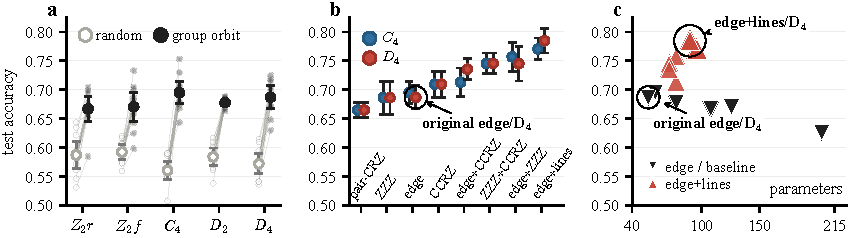
\includegraphics[width=\textwidth]{images/fig_controls.pdf}
\caption{Controls und Ablationen. Links: Random sharing schlägt symmetry-aware sharing nicht. Mitte: Oracle-inspirierte Ablation bei 600 Trainingsbeispielen. Rechts: Accuracy ist nicht allein durch Parameterzahl erklärbar; task-aligned equivariant geometry verschiebt das Modell in einen anderen Leistungsbereich.}
\label{fig:controls}
\end{figure}

Der Parametervergleich ist wichtig. Das beste $D_4$-Edge-plus-Line-Modell hat 90 Parameter, also mehr als das Edge/$D_4$-Modell mit 54 Parametern, aber immer noch deutlich weniger als der unbeschränkte Edge-Baseline mit 204 Parametern. Die Verbesserung ist also nicht einfach \emph{mehr Parameter}. Gleichzeitig wäre es auch falsch zu sagen, dass weniger Parameter immer besser sind. Die richtige Beschreibung lautet: Die zusätzlichen Parameter liegen an der richtigen Stelle, nämlich auf äquivariant geteilten Gewinnlinien.

\subsection{Deterministischer Oracle als Sanity Check}\label{subsec:rule-oracle}

Weil Tic-Tac-Toe regelbasiert lösbar ist, haben wir zusätzlich einen deterministischen Oracle implementiert. Dieser prüft die klassischen Gewinnbedingungen direkt und erreicht auf allen 5478 legalen Zuständen 100\% Accuracy bei null trainierbaren Parametern. Das ist kein konkurrierendes VQLM, sondern eine Sanity-Referenz. Es zeigt, dass die Labels eindeutig und die Aufgabe nicht intrinsisch schwierig sind. Der Abstand zwischen $0.80$ und $1.00$ ist daher kein Problem der Daten, sondern ein Problem der gewählten variationalen Architektur und Optimierung.

Diese Beobachtung hilft, den wissenschaftlichen Claim sauber zu formulieren. Wir zeigen nicht, dass ein Quantenmodell Tic-Tac-Toe optimal löst. Wir zeigen, dass eine bessere äquivariante Architektur einen großen Teil des Abstands zwischen dem Meyer-artigen Baseline-Ansatz und dem trivialen Regel-Oracle schließt.

\section{Diskussion}\label{sec:diskussion}

\subsection{Was bedeutet ``When to Break Symmetry'' hier?}\label{subsec:break}

Der ursprüngliche Arbeitstitel \emph{When to Break Symmetry} suggeriert, dass die beste Strategie möglicherweise darin besteht, volle $D_4$-Symmetrie bewusst zu brechen. Die aktuellen Resultate stützen diesen starken Claim nur eingeschränkt. $C_4$ ist kompetitiv und in kleinen Datenregimen punktuell besser, aber es schlägt $D_4$ nicht robust. Deshalb wäre die harte Aussage \emph{man sollte volle Symmetrie brechen} wissenschaftlich zu stark.

Eine bessere Formulierung ist: \emph{When to relax or redesign symmetry}. Partielle Symmetrie zeigt, dass der Symmetriegrad eine sinnvolle Modellwahlachse ist. Die winning-line-Ergebnisse zeigen aber, dass der stärkere Hebel darin liegt, die äquivariante Architektur selbst zu verbessern. Man muss $D_4$ nicht brechen, um $D_4$ zu schlagen; man kann innerhalb von $D_4$ bessere Gates platzieren.

\subsection{Symmetrie ist nicht gleich Parameterreduktion}\label{subsec:notparams}

Die Random-Sharing-Ergebnisse sind der wichtigste Kontrollpunkt der Arbeit. Ohne sie wäre der Claim schwach. Wenn random tying mit gleicher Parameterzahl denselben Effekt hätte, dann wäre Symmetrie nur eine dekorative Erklärung für Regularisierung. Die Daten zeigen das Gegenteil. Symmetry-aware sharing ist deutlich besser als random sharing. Das spricht dafür, dass die Gruppenstruktur selbst relevant ist.

Gleichzeitig zeigen die Oracle-inspirierten Gates, dass Parameterzahl allein auch in die andere Richtung nicht erklärt. Das beste Modell hat mehr Parameter als Edge/$D_4$, aber weniger als edge/none. Es gewinnt nicht durch maximale Expressivität, sondern durch strukturierte Expressivität. Das ist die zentrale Lehre für Praktiker: Wenn eine Aufgabe bekannte Motive besitzt, sollte man nicht nur Parameter teilen, sondern auch Gates so wählen, dass diese Motive als Interaktionen verfügbar sind.

\subsection{Warum Winning-Line-Gates sinnvoll sind}\label{subsec:whyline}

Tic-Tac-Toe ist ein gutes Beispiel, weil die relevante Struktur offensichtlich ist. Ein Sieg entsteht aus drei gleichen Zeichen in einer Zeile, Spalte oder Diagonale. Ein rein paarbasierter Edge-Ansatz muss solche Dreiermotive indirekt darstellen. Winning-Line-Gates geben dem Modell dagegen direkte trainierbare Interaktionen auf genau diesen Triples. Das ist nicht ad hoc im schlechten Sinn, sondern task-aligned im selben Sinn, in dem eine Faltung für Bilddaten task-aligned ist: Die Architektur spiegelt die lokale Struktur des Problems wider.

Die Analogie zu klassischen Modellen ist hilfreich. Ein CNN ist nicht nur ein MLP mit weniger Parametern. Es stellt lokale, geteilte Filter bereit, die zur Bildgeometrie passen. Entsprechend ist unser Edge-plus-Line-VQLM nicht nur ein Edge-VQLM mit mehr Parametern. Es stellt äquivariant geteilte Dreierinteraktionen bereit, die zur Gewinnregel passen.

\subsection{Grenzen der Ergebnisse}\label{subsec:limits}

Die Ergebnisse bleiben finite-seed Simulationen. Die wichtigsten Sweeps verwenden fünf Seeds. Für eine finale Publikation sollten die Headline-Vergleiche mit 10 bis 20 Seeds wiederholt werden. Außerdem ist die Architektur Meyer-artig, aber keine Byte-für-Byte-Reproduktion des Originalcodes. Die Richtung des Meyer-Effekts wird reproduziert, die absoluten Zahlen sollten jedoch als Ergebnis unserer Implementierung verstanden werden.

Eine weitere Grenze ist die Aufgabengröße. Tic-Tac-Toe ist klein und vollständig enumerierbar. Das ist für kontrollierte Experimente ein Vorteil, aber es bedeutet nicht automatisch, dass dieselbe Architekturidee auf größere Aufgaben skaliert. Der übertragbare Teil ist nicht das konkrete Winning-Line-Gate, sondern das Prinzip: Wenn eine symmetrische Aufgabe bekannte lokale oder relationale Motive besitzt, sollte ein äquivariantes VQLM diese Motive direkt als trainierbare Interaktionen anbieten.

\subsection{Soft Symmetry als Ausblick}\label{subsec:soft}

Die ursprüngliche Idee einer Soft Gate Symmetrization bleibt als Ausblick interessant. Man könnte einen Generator $G$ in einen symmetrischen und einen symmetry-breaking Anteil zerlegen:
\begin{equation}
G_\alpha=\Pi_{\mathrm{sym}}(G)+\alpha\bigl(G-\Pi_{\mathrm{sym}}(G)\bigr),
\quad \alpha\in[0,1].
\label{eq:soft}
\end{equation}
Für $\alpha=0$ erhält man harte Äquivarianz, für $\alpha=1$ den freien Generator. Eine zukünftige Arbeit könnte damit kontrolliert untersuchen, ob der optimale Symmetriegrad mit einem künstlich eingeführten Symmetriebruch wandert.

Die aktuellen Resultate zeigen jedoch, dass vor dieser kontinuierlichen Frage bereits eine architektonische Frage steht. Wenn ein hart äquivariantes Modell schlecht genug ist, kann der Grund nicht nur zu viel Symmetrie sein. Der Grund kann auch sein, dass die falschen äquivarianten Interaktionen angeboten werden. Genau das legt der Gewinn der Winning-Line-Gates nahe.

\section{Fazit}\label{sec:fazit}

Diese Arbeit rekonstruiert Meyer et al. als Ausgangspunkt für eine breitere Sicht auf Symmetrie in Variational Quantum Learning. Die Reproduktion bestätigt qualitativ: volle $D_4$-Äquivarianz verbessert die Test Accuracy gegenüber keiner Symmetrie und reduziert den Generalization Gap. Die Untergruppenexperimente zeigen, dass partielle Äquivarianz eine sinnvolle Modellwahlachse ist; insbesondere $C_4$ erreicht fast dieselbe Leistung wie $D_4$, ohne robust besser zu sein. Der Random-Sharing-Control zeigt, dass der Effekt nicht bloß durch weniger Parameter erklärt werden kann.

Der wichtigste neue Befund ist die task-aligned äquivariante Architektur. Durch zusätzliche Gates auf den acht Gewinnlinien steigt die Test Accuracy im besten $D_4$-Modell von etwa $0.69$ auf etwa $0.80$. Das Modell bleibt dabei äquivariant. Der stärkste Claim ist daher nicht, dass man Symmetrie brechen muss. Der stärkste Claim ist: Sobald Symmetrie eingebaut ist, sollte man den äquivarianten Designraum weiter nutzen, um Gates an die Struktur der Aufgabe anzupassen.

Für zukünftige VQLM-Benchmarks ergibt sich daraus eine konkrete Empfehlung. Eine bekannte Symmetrie sollte nicht nur als Parameter-Sharing-Regel verwendet werden. Sie sollte als Sprache dienen, in der man task-aligned Gates konstruiert: lokale Motive, relationale Muster, konservierte Größen oder kombinatorische Substrukturen. In diesem Sinn erweitert die Arbeit Meyer et al. natürlich: Meyer et al. zeigen, dass Symmetrie hilft; diese Arbeit zeigt, dass die Wahl der symmetrieverträglichen Interaktionen mindestens ebenso wichtig sein kann.

\clearpage
\section*{Formale Angaben}
\addcontentsline{toc}{section}{Formale Angaben}

\noindent\textcolor{red}{\Large Wortanzahl fachlicher Haupttext: \textbf{3294}}

\vspace{0.3cm}
\noindent\textcolor{red}{\Large Zeichenanzahl ohne Leerzeichen: \textbf{22554}}

\vspace{0.3cm}
\noindent\textcolor{red}{\Large Zeichenanzahl mit Leerzeichen: \textbf{26425}}

\vspace{0.5cm}
\noindent\emph{Hinweis:} Die Zählung bezieht sich auf den fachlichen Haupttext in \texttt{contents.tex} bis einschließlich Fazit, inklusive Überschriften und Bildunterschriften, aber ohne LaTeX-Kommandos, Literaturbefehle, Tabellenkörper und Gleichungen. Der automatische \texttt{texcount}-Block der Vorlage wurde ersetzt, weil \texttt{texcount} in der aktuellen lokalen TeX-Installation nicht verfügbar ist.

\clearpage
\section*{Eigenständigkeitserklärung}
\noindent Hiermit bestätige ich, dass ich die vorliegende Arbeit selbstständig verfasst und keine anderen als die angegebenen Hilfsmittel benutzt habe. Die Stellen der Arbeit, die dem Wortlaut oder dem Sinn nach anderen Werken entnommen sind, wurden unter Angabe der Quelle kenntlich gemacht.

\vspace{1cm}

\noindent Unterschrift

\clearpage


% Literatur
\bibliography{references}
\bibliographystyle{plain}

% Template notes are kept in the project as hinweise.tex, but are not included in the final paper.
% \clearpage
\section*{Hinweise}
Nachfolgend ein paar Hinweise und Lessons Learned aus der Vergangenheit.

\subsection*{Inhalt}
\begin{itemize}
    \item Logischen Zusammenhang zwischen den einzelnen Abschnitten herstellen
    \item Offene Enden/reine Definitionssalate verleiten Betreuer zu Fragen. Vorsichtig sein, wenn das Wissen nicht über die reine Definition hinausgeht.
    \item Achte auf eine gleichmäßige und dichte Darstellung des Inhalts. Der Platz sollte sinnvoll genutzt werden, keine inhaltsleeren oder zu lange/zu kurze Texte.
\end{itemize}

\subsection*{Form}
\begin{itemize}
    \item Schreibfehler und Kommasetzungsfehler sollten Dank moderner Tools der Vergangenheit angehören. Mehr als 1 Fehler pro Seite führen zur Abwertung, die sich an der Anzahl der Fehler orientiert. Es gibt keine „Folgefehler“ für konsequent falsche Rechtschreibung.
    \item Bilder sollen in ausreichender Auflösung eingebunden werden (besser: Vektor-Grafik, noch besser: tikz).
    \item Jede Section sollte ein Label haben {\lstset{basicstyle=\ttfamily\bfseries}\lstinline|\label{sec:name}|}.
    \item Für den Titel der Arbeit und die Abschnittstitel \textit{titlecase} verwenden
    \item Keine alleinstehenden Unterkapitel. Mind. 2 Unterkapitel pro Ebene verwenden.
\end{itemize}

\subsection*{Sprache}
\begin{itemize}
    \item Wortstellung beachten: Subjekt, Prädikat und Objekt. Im Zweifelsfall Korrektur lesen lassen.
    \item Jeder Satz soll einen Zweck erfüllen und Informationen transportieren (keine Hohlphrasen!)
    \item Kurze Sätze sind leichter verständlich als lange, verschachtelte Sätze. Naturwissenschaftliche Arbeiten sollen Informationen vermitteln.
    \item Kommunikation soll intersubjektiv erfolgen. (Der Betreuer und jeder andere Leser, soll ansatzweise und in angemessener Zeit verstehen können, was ihr da schreibt.)
    \item Fachbegriffe dürfen auf Englisch verwendet werden, müssen aber eingeführt werden. Beispiel: „Maschinelles Lernen (sogenanntes englisches Machine Learning (ML)) ist toll.“
    \item Englische Fachbegriffe werden im Deutschen groß geschrieben!
    \item Wissenschaftliche Texte werden im Deutsch im Passiv geschrieben.
    \item Verwendet Begriffe einheitlich, das heißt keine verschiedenen Begriffe für ein und dieselbe Sache verwenden wie beispielsweise „State“, „Zustand“, „Status“ oder Ähnliches. Entscheidet euch für eine Variante. Es geht nicht darum möglichst kreativ sondern deutlich zu schreiben.
    \item Akronyme sollen einmal im Hauptteil der Arbeit (nicht in Überschriften, nicht im Abstract) eingeführt und danach konsequent verwendet werden. Was geeignete Akronyme sind und was nicht, kann euren Quellen entnommen werden. Beispielsweise: „Machine Learning (ML) ist toll. Insbesondere hat ML den Vorteil, dass\ldots{}“. Das Latex-Package \textit{glossaries} kann automatisiert beim ersten Verwenden eines Fachbegriffs die Abkürzung einführen:
    \begin{verbatim}
    \newglossaryentry{LED}
    {
      name={LED},
      description={light emitting diode},
      first={\glsentrydesc{LED} (\glsentrytext{LED})},
      plural={LEDs},
      descriptionplural={light emitting diodes},
      firstplural={\glsentrydescplural{LED} (\glsentryplural{LED})}
    }
    \end{verbatim}
    Verwendung: {\lstset{basicstyle=\ttfamily\bfseries}\lstinline|\gls{LED}|} und im Plural {\lstset{basicstyle=\ttfamily\bfseries}\lstinline|\glspl{LED}|}.
\end{itemize}

\subsection*{Zitierweise}
\begin{itemize}
    \item Zitate von Websites sind nicht angebracht; verwendet nur Peer-Reviewed-Dokumente.
    \item Zitate sollen mit der vordefinierten Zitierweise vorgenommen werden. Zitierstil des Templates nicht ändern!
    \item Eine direkte Übersetzung muss auch zitiert werden.
    \item Wenn Elemente (Bilder, Tabellen, Code) von Dritten (aus der Literatur) verwendet werden, muss die Quelle bei jeder Verwendung explizit zitiert werden.
    \item Blog-Artikel können meist nicht zitiert werden. Ausnahmen bilden Grafiken und andere Elemente, hier muss eine manuell eine korrekte Zitation angelegt werden. Prüft die Korrektheit!
    \item  Zitate mit Seitenverweis müssen auch als solche ausgeführt werden (z B [2, Seite 44] o.ä.)
\end{itemize}

\subsection*{Querverweise}
\begin{itemize}
    \item  Jedes Element (Abbildung, Tabelle, Diagramm, Code, etc.) muss zur wissenschaftlichen Auseinandersetzung mit dem Thema erforderlich sein.
    \item Der Text muss sich mit dem Element auseinandersetzen (es mindestens einmal geeignet referenzieren) und es muss die Argumentation stützen. Es reicht nicht aus, dass das Element gut zum Text passt oder die Arbeit optisch aufwertet.
    \item Befehl für Querverweise {\lstset{basicstyle=\ttfamily\bfseries}\lstinline|\cref{label}|}. Im Vergleich zum normalen {\lstset{basicstyle=\ttfamily\bfseries}\lstinline|\ref|} Befehl, wird mit {\lstset{basicstyle=\ttfamily\bfseries}\lstinline|\cref|} wird auch direkt der Verweis-Typ mit ausgegeben. Beispiel {\lstset{basicstyle=\ttfamily\bfseries}\lstinline|\cref|}: \cref{fig:karate}, {\lstset{basicstyle=\ttfamily\bfseries}\lstinline|\ref|}:~\ref{fig:karate}. Der Verweistyp passt sich automatisch dem referenzierten Inhalt an. Es können auch Sub-Figures referenziert werden: \cref{fig:karate1}, \cref{fig:karate2}.
\end{itemize}
\end{document}
